\begin{pastexam}[label={px:gk3-109-ds-04}]{高考三級資訊處理 109 年 第四題}
（申論；30 分）

若我們用相鄰矩陣（Adjacency Matrix）$M$ 來表示圖一中的無向圖 $G = (V, E)$，請考慮下面的問題：
\begin{center}
\begin{tikzpicture}[x=1.35cm, y=1.1cm,
  v/.style={circle, draw, thick, minimum size=5.5mm, inner sep=0pt, font=\small\itshape\bfseries}]
\node[v] (d) at (0,2) {d};
\node[v] (a) at (1.5,2) {a};
\node[v] (e) at (3,2) {e};
\node[v] (h) at (0,1) {h};
\node[v] (g) at (1.5,1) {g};
\node[v] (b) at (3,1) {b};
\node[v] (c) at (1.5,0) {c};
\node[v] (f) at (3,0) {f};
\draw[very thick] (d)--(a) (a)--(e) (d)--(h) (h)--(a) (a)--(g) (a)--(b) (e)--(b)
  (g)--(b) (g)--(c) (c)--(b) (b)--(f) (c)--(f);
\node[font=\small] at (1.5,-0.55) {圖一、無向圖 $G = (V, E)$};
\end{tikzpicture}
\end{center}
\begin{itemize}[leftmargin=2em, labelsep=0.3em, itemsep=2pt]
\item[㈠] 對於無向圖 $G = (V, E)$：（12 分）
\begin{itemize}[leftmargin=2em, labelsep=0.3em, itemsep=1pt]
\item[⑴] 請給出對應的相鄰矩陣 $M$。
\item[⑵] 以字母順序為考量進行深度優先搜尋（Depth-First Search, DFS），請由節點 $a$ 開始，描述此
深度優先搜尋所產生的深度優先樹（DF-tree）。
\end{itemize}
\item[㈡] 請說明在用相鄰矩陣（Adjacency Matrix）表示的無向圖上，進行深度優先搜尋的時間複雜度，其中
節點與邊的數量分別為 $|V| = n$ 與 $|E| = m$。（8 分）
\item[㈢] 若將圖一無向圖 $G = (V, E)$ 中的邊給予方向成為如圖二中的有向圖（Directed Graph）$G'$：
（10 分）
\begin{center}
\begin{tikzpicture}[x=1.35cm, y=1.1cm, >=Stealth,
  v/.style={circle, draw, thick, minimum size=5.5mm, inner sep=0pt, font=\small\itshape\bfseries}]
\node[v] (d) at (0,2) {d};
\node[v] (a) at (1.5,2) {a};
\node[v] (e) at (3,2) {e};
\node[v] (h) at (0,1) {h};
\node[v] (g) at (1.5,1) {g};
\node[v] (b) at (3,1) {b};
\node[v] (c) at (1.5,0) {c};
\node[v] (f) at (3,0) {f};
\draw[->, very thick] (a)--(d);
\draw[->, very thick] (e)--(a);
\draw[->, very thick] (d)--(h);
\draw[->, very thick] (a)--(h);
\draw[->, very thick] (a)--(g);
\draw[->, very thick] (b)--(a);
\draw[->, very thick] (b)--(e);
\draw[->, very thick] (b)--(g);
\draw[->, very thick] (c)--(g);
\draw[->, very thick] (c)--(b);
\draw[->, very thick] (b)--(f);
\draw[->, very thick] (c)--(f);
\node[font=\small] at (1.5,-0.55) {圖二、有向圖 $G'$};
\end{tikzpicture}
\end{center}
\begin{itemize}[leftmargin=2em, labelsep=0.3em, itemsep=1pt]
\item[⑴] 有向圖 $G'$ 沒有迴圈（Cycle），是一個無迴圈有向圖（Directed Acyclic Graph, DAG），所以存在
節點的拓樸排序（Topological Sort），請對 $G'$ 給出一個拓樸排序（Topological Sort）。
\item[⑵] 請給一個方法來判斷一個有向圖是否沒有迴圈。
\end{itemize}
\end{itemize}
\end{pastexam}

\begin{pastsoln}
圖一有 $8$ 個頂點、$12$ 條邊：
$a$--$b$、$a$--$d$、$a$--$e$、$a$--$g$、$a$--$h$、$b$--$c$、$b$--$e$、$b$--$f$、$b$--$g$、$c$--$f$、
$c$--$g$、$d$--$h$。 主要考深度優先搜尋，㈢的拓樸排序屬資結書第~22~章。

\textbf{㈠⑴} 列、行都依 $a, b, \ldots, h$ 的順序，有邊記 $1$。 無向圖的矩陣對稱，對角線為 $0$：
\[
M = \begin{array}{c|cccccccc}
 & a & b & c & d & e & f & g & h \\ \hline
a & 0 & 1 & 0 & 1 & 1 & 0 & 1 & 1 \\
b & 1 & 0 & 1 & 0 & 1 & 1 & 1 & 0 \\
c & 0 & 1 & 0 & 0 & 0 & 1 & 1 & 0 \\
d & 1 & 0 & 0 & 0 & 0 & 0 & 0 & 1 \\
e & 1 & 1 & 0 & 0 & 0 & 0 & 0 & 0 \\
f & 0 & 1 & 1 & 0 & 0 & 0 & 0 & 0 \\
g & 1 & 1 & 1 & 0 & 0 & 0 & 0 & 0 \\
h & 1 & 0 & 0 & 1 & 0 & 0 & 0 & 0
\end{array}
\]
每列 $1$ 的個數就是度數：$5, 5, 3, 2, 2, 2, 3, 2$，總和 $24 = 2 \times 12$。

\textbf{㈠⑵} 從 $a$ 開始，每次在目前頂點的鄰居中，依字母順序找第一個還沒拜訪的往下走；沒有就
退回上一層（資結書第~21.4~節）。
\begin{center}
\small
\begin{tabular}{lll}
\toprule
目前頂點 & 依字母順序看鄰居 & 動作 \\
\midrule
$a$ & $b, d, e, g, h$ & 走到 $b$（樹邊 $a$--$b$） \\
$b$ & $a$（已拜訪）, $c$ & 走到 $c$（樹邊 $b$--$c$） \\
$c$ & $b$（已）, $f$ & 走到 $f$（樹邊 $c$--$f$） \\
$f$ & $b$, $c$ 都已拜訪 & 退回 $c$ \\
$c$ & $g$ & 走到 $g$（樹邊 $c$--$g$） \\
$g$ & $a, b, c$ 都已拜訪 & 退回 $c$，$c$ 的鄰居看完，退回 $b$ \\
$b$ & $e$ & 走到 $e$（樹邊 $b$--$e$） \\
$e$ & $a, b$ 都已拜訪 & 退回 $b$；$b$ 剩下的 $f, g$ 已拜訪，退回 $a$ \\
$a$ & $d$ & 走到 $d$（樹邊 $a$--$d$） \\
$d$ & $a$（已）, $h$ & 走到 $h$（樹邊 $d$--$h$） \\
$h$ & $a, d$ 都已拜訪 & 退回 $d$、$a$；$a$ 剩下的 $e, g, h$ 已拜訪，結束 \\
\bottomrule
\end{tabular}
\end{center}
拜訪順序 $a, b, c, f, g, e, d, h$。 深度優先樹以 $a$ 為根，$7$ 條樹邊：
\begin{center}
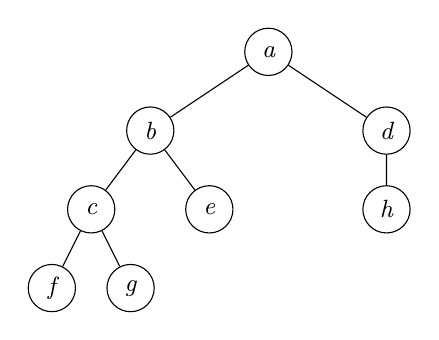
\begin{tikzpicture}[level distance=10mm,
  level 1/.style={sibling distance=30mm}, level 2/.style={sibling distance=15mm},
  level 3/.style={sibling distance=10mm},
  every node/.style={circle, draw, minimum size=6mm, inner sep=0pt, font=\small\itshape}]
\node {a}
  child {node {b} child {node {c} child {node {f}} child {node {g}}} child {node {e}}}
  child {node {d} child {node {h}}};
\end{tikzpicture}
\end{center}
其餘 $5$ 條邊 $a$--$e$、$a$--$g$、$a$--$h$、$b$--$f$、$b$--$g$ 都是後向邊（連到祖先），無向圖的 DFS
沒有交叉邊（資結書定理~21.8）。

\textbf{㈡ 時間複雜度 $\Theta(n^2)$。} DFS 對每個頂點恰好拜訪一次（拜訪時標記，之後不再進入）。
拜訪頂點 $u$ 時要找出它所有的鄰居，在相鄰矩陣上只能把第 $u$ 列的 $n$ 格全部看過，$\Theta(n)$。
$n$ 個頂點合計 $n \cdot \Theta(n) = \Theta(n^2)$，加上初始化標記 $\Theta(n)$，總共 $\Theta(n^2)$，
\textbf{和邊數 $m$ 無關}。 若改用相鄰串列，找鄰居只要看實際的鄰居，總共 $\Theta(n + m)$；稀疏圖
（$m \ll n^2$）時相鄰串列快得多（資結書第~21.2~節）。

\textbf{㈢⑴} 用 Kahn 方法（資結書第~22.1~節）：反覆取出入度為 $0$ 的頂點並刪去它的出邊。 $G'$ 的
邊：$a \to d$、$a \to g$、$a \to h$、$b \to a$、$b \to e$、$b \to f$、$b \to g$、$c \to b$、
$c \to f$、$c \to g$、$d \to h$、$e \to a$。 初始入度：$a{:}2$、$b{:}1$、$c{:}0$、$d{:}1$、$e{:}1$、
$f{:}2$、$g{:}3$、$h{:}2$。 有多個入度 $0$ 的頂點時取字母最小的：
\begin{center}
\small
\begin{tabular}{clll}
\toprule
步 & 取出 & 入度變化 & 入度為 $0$ 的候選 \\
\midrule
1 & $c$ & $b{:}0$, $f{:}1$, $g{:}2$ & $b$ \\
2 & $b$ & $a{:}1$, $e{:}0$, $f{:}0$, $g{:}1$ & $e, f$ \\
3 & $e$ & $a{:}0$ & $a, f$ \\
4 & $a$ & $d{:}0$, $g{:}0$, $h{:}1$ & $d, f, g$ \\
5 & $d$ & $h{:}0$ & $f, g, h$ \\
6 & $f$ & — & $g, h$ \\
7 & $g$ & — & $h$ \\
8 & $h$ & — & （空） \\
\bottomrule
\end{tabular}
\end{center}
一個拓樸排序是
\[
c,\ b,\ e,\ a,\ d,\ f,\ g,\ h .
\]
逐邊檢查都是由前指向後，例如 $c \to b$、$b \to e \to a \to d \to h$、$a \to g$。 拓樸排序不唯一
（$G'$ 共有 $18$ 種），例如 $c, b, f, e, a, g, d, h$ 也對；但 $c$ 一定第一（唯一入度 $0$ 的頂點），
$b$ 一定第二。

\textbf{㈢⑵ 判斷有向圖有沒有迴圈}，兩種方法擇一（時間都是相鄰串列 $\Theta(n + m)$）：
\begin{itemize}[nosep]
\item \textbf{Kahn 方法}：照⑴的步驟做，若所有 $n$ 個頂點都被取出，圖沒有迴圈；若做到某一步已沒有
入度 $0$ 的頂點、卻還有頂點沒被取出，剩下的頂點入度都 $\ge 1$，從任一個沿著入邊往回走一定會重複，
所以有迴圈（資結書定理~22.3）。
\item \textbf{DFS 三色法}：頂點分白（未拜訪）、灰（在目前的遞迴堆疊上）、黑（已完成）。 DFS 時若從
灰色頂點 $u$ 看到另一個\textbf{灰色}頂點 $v$（後向邊），$v$ 是 $u$ 的祖先，$v \leadsto u \to v$ 是一個
迴圈；整個 DFS 都沒遇到後向邊，圖就沒有迴圈（資結書定理~21.10）。
\end{itemize}
\end{pastsoln}
